\section{Continuous-Time Fourier Transform}

\subsection{Introduction}
\begin{frame}{Introduction}
    \begin{itemize}[<+->]
      \item Using the Fourier techniques we can obtain the frequency-domain representation of signals.
      \item We use Fourier series for periodic signals, and Fourier transform for aperiodic signals.
      \item Each of these have continuous-time and discrete-time versions:
        \begin{enumerate}
            \item Continuous-time Fourier series
            \item Continuous-time Fourier transform
            \item Discrete-time Fourier series
            \item Discrete-time Fourier transform
        \end{enumerate}
      \item In this part of the course, we will concentrate on how to actually compute continuous-time Fourier series and transform. Later, after we study liner, time-invariant (LTI) systems, we will study the conceptual aspects of Fourier techniques.
    \end{itemize}
\end{frame}

\begin{frame}{Fourier Transform}
    \begin{itemize}[<+->]
          \item In the last lecture, we represented a periodic signal as a linear combination of complex exponentials.
          \item We use Fourier transform to represent aperiodic signals. A larger class of signals, including all signals with finite energy, can be represented through a linear combination of complex exponentials.
          \item Whereas for periodic signals the complex exponential building blocks are harmonically related, for aperiodic signals they are infinitesimally close in frequency, and the representation in terms of a linear combination takes the form of an integral rather than a sum.
          \item The resulting spectrum of coefficients in this representation is called the Fourier transform.
          \item The synthesis integral itself, which uses these coefficients to represent the signal as a linear combination of complex exponentials, is called the inverse Fourier transform.
      \end{itemize}
\end{frame}


\subsection{Development of the Fourier Transform Representation}

\begin{frame}[plain]{Fourier Series Representation for Square Wave}
        The continuous-time periodic square wave, sketched below, is defined over one period as
        \begin{equation*}
            x(t) = \begin{cases}
                1, & |t| <T_1,\\
                0, & T_1 < |t| < T/2,
            \end{cases}
        \end{equation*}
        This signal is periodically repeats with fundamental period $T$ and fundamental frequency $\omega_0 = 2\pi/T$.
    \mode<beamer>
    {
        \begin{figure}
          \centering
          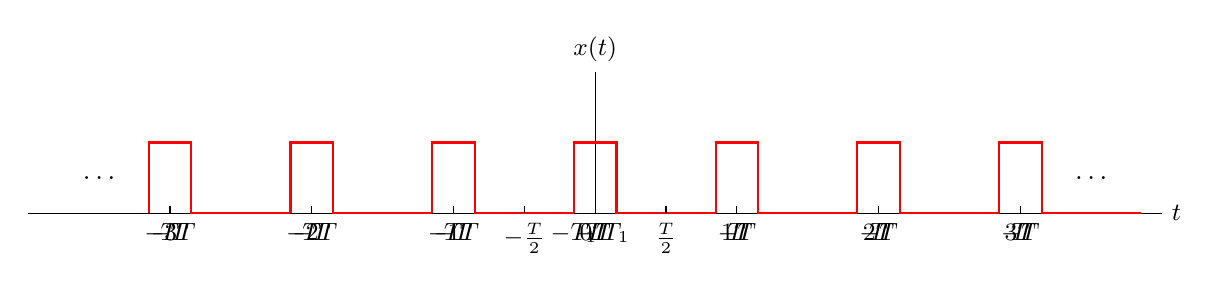
\begin{tikzpicture}[scale=0.9]
	\def\xmin{-7}
	\def\xmax{7}
	\def\ymin{0}
	\def\ymax{2}
	\def\period{2.0}
	\def\T1{0.3}
	\def\A{1}
	
	\edef\pulse{|- ++(2*\T1, \A) |- ++( \period - 2*\T1, -\A)}

	
	\draw (\xmin-1, 0) --(\xmax+1, 0) node[anchor=west] {\small $t$};
	\draw (0, \ymin) --(0, \ymax) node[anchor=south] {\small $x(t)$};
		\foreach \x in {-3, -2, ..., 3}
		{
			\pgfmathmultiply{\period}{\x}
			\edef\position{\pgfmathresult}
			\ifthenelse{\x=0 \OR \x=1 \OR \x=-1}
			{
				%\node at (\position, 0) [anchor=north] {\small $0$};
			}
			{
				
				\node at (\position, 0) [anchor=north] {\small $\x T$};
			}
			\ifthenelse{ \x=1 }
			{
				\node at (\position, 0) [anchor=north] {\small $T$};
			}
			{
			}
			
			\ifthenelse{ \x=-1 }
			{
				\node at (\position, 0) [anchor=north] {\small $-T$};
			}
			{
			}			
			\draw[thick, red] (\position-\T1, 0) \pulse;	
			\draw (\position, 0) -- ++(0,0.1);
			%\pulse{3}{0.4};		
		}
		
		\node at (-\T1, 0) [anchor=north] {\small $-T_1$};
		\node at (\T1, 0) [anchor=north] {\small $T_1$};
		\node at (-\period/2, 0) [anchor=north] {\small $-\frac{T}{2}$};
		\node at (\period/2, 0) [anchor=north] {\small $\frac{T}{2}$};
		\draw (-\period/2, 0) -- ++(0,0.1);
		\draw (\period/2, 0) -- ++(0,0.1);

		\node at (\xmin, \A/2) {$\dots$};
		\node at (\xmax, \A/2) {$\dots$};
\end{tikzpicture}

          \caption{Periodic square wave}\label{fi:example02_periodic_square_wave }
        \end{figure}
    }
\end{frame}



\begin{frame}
    The Fourier series coefficients $a_k$ of this wave are
    \begin{equation}\label{eq:square_fs}
        a_k = \frac{2\sin(k\omega_0T_1)}{k\omega_0T}
    \end{equation}
    We plotted this for a fixed value of $T_1$ and several values of $T$ (shown in the next slide). An alternative wave of interpreting eq. \ref{eq:square_fs} is as samples of an envelope function:
    \begin{equation*}
        Ta_k = \left.\frac{2\sin(\omega T_1)}{\omega}\right|_{\omega=k\omega_0}
    \end{equation*}
    For fixed $T_1$, the envelope of $Ta_k$ is independent of $T$.

\end{frame}

\begin{frame}[plain,t]
    \begin{columns}
        \column{0.8\textwidth}
        {
        \begin{figure}
          \centering
          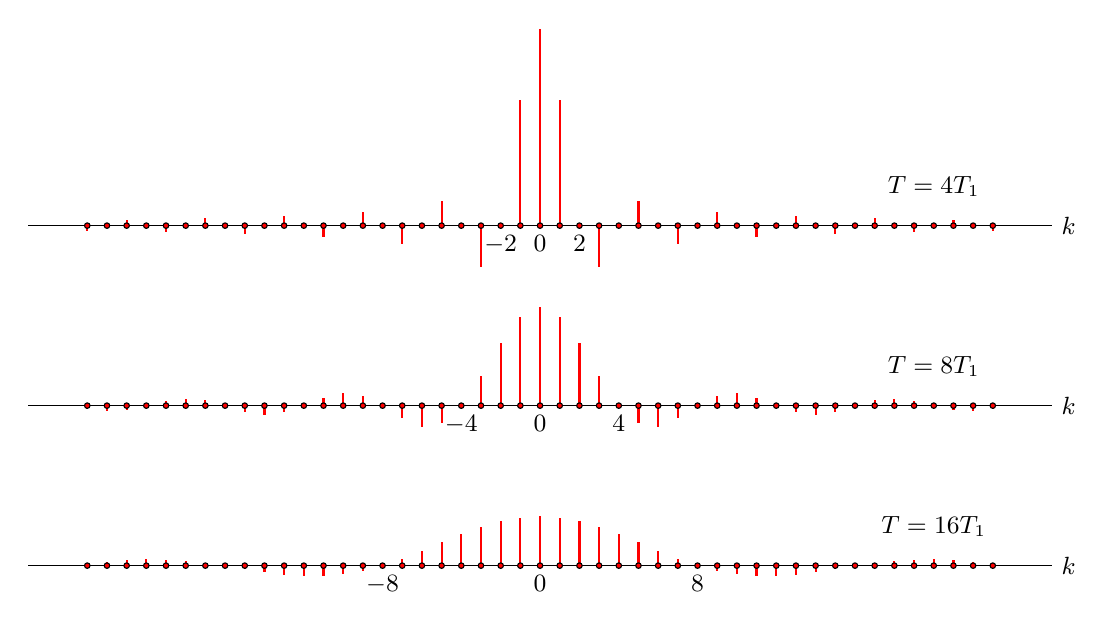
\begin{tikzpicture}[scale=0.5]
	\def\w{{-23,-22,-21,-20,-19,-18,-17,-16,-15,-14,-13,-12,-11,-10,-9,-8,-7,-6,-5,-4,-3,-2,-1,0,1,2,3,4,5,6,7,8,9,10,11,12,13,14,15,16,17,18,19,20,21,22,23}}
	\def\akmag{{-0.013840,0.000000,0.015158,-0.000000,-0.016753,0.000000,0.018724,-0.000000,-0.021221,0.000000,0.024485,-0.000000,-0.028937,0.000000,0.035368,-0.000000,-0.045473,0.000000,0.063662,-0.000000,-0.106103,0.000000,0.318310,0.500000,0.318310,0.000000,-0.106103,-0.000000,0.063662,0.000000,-0.045473,-0.000000,0.035368,0.000000,-0.028937,-0.000000,0.024485,0.000000,-0.021221,-0.000000,0.018724,0.000000,-0.016753,-0.000000,0.015158,0.000000,-0.013840}}


	\begin{scope}	
		\draw (-13, 0) -- (13,0) node[anchor=west] {\small $k$};
		\foreach \k in {-2, 0, 2}
		{
			\node at (\k/2, 0) [anchor=north] {\small $\k$};
		}
		%\node at (0,5) [anchor=south] {\small $Ta_k$};
		
		\foreach \k in {0,1, ..., 46}
		{
			\pgfmathparse{\w[\k]/2}
			\edef\wk{\pgfmathresult}
			\pgfmathparse{\akmag[\k]}
			\edef\akmagk{\pgfmathresult}	
			\draw[thick, red] (\wk, 0) -- ++(0,10*\akmagk);% node [anchor=south] {\small $\akmagk$};
			\ifthenelse{\lengthtest{0 pt = \akmagk pt}}{\draw[fill=red]  (\wk,0) circle (2pt);}{}
		}
			\node at (10, 1) {\small $T= 4T_1$};		
	\end{scope}

%\pause
\def\akmag{{-0.009786,-0.014469,-0.010718,0.000000,0.011846,0.017684,0.013240,-0.000000,-0.015005,-0.022736,-0.017314,0.000000,0.020462,0.031831,0.025009,-0.000000,-0.032154,-0.053052,-0.045016,0.000000,0.075026,0.159155,0.225079,0.250000,0.225079,0.159155,0.075026,0.000000,-0.045016,-0.053052,-0.032154,-0.000000,0.025009,0.031831,0.020462,0.000000,-0.017314,-0.022736,-0.015005,-0.000000,0.013240,0.017684,0.011846,0.000000,-0.010718,-0.014469,-0.009786}}


	\begin{scope}[yshift=-1.8in]
		\draw (-13, 0) -- (13,0) node[anchor=west] {\small $k$};
		\foreach \k in {-4, 0, 4}
		{
			\node at (\k/2, 0) [anchor=north] {\small $\k$};
		}
		%\node at (0,5) [anchor=south] {\small $Ta_k$};
		
		\foreach \k in {0,1, ..., 46}
		{
			\pgfmathparse{\w[\k]/2}
			\edef\wk{\pgfmathresult}
			\pgfmathparse{\akmag[\k]}
			\edef\akmagk{\pgfmathresult}	
			\draw[thick, red] (\wk, 0) -- ++(0,10*\akmagk);% node [anchor=south] {\small $\akmagk$};
			\ifthenelse{\lengthtest{0 pt = \akmagk pt}}{\draw[fill=red]  (\wk,0) circle (2pt);}{}		
		}
			\node at (10, 1) {\small $T= 8T_1$};			
	\end{scope}
%\pause
\def\akmag{{0.005296,0.010231,0.014004,0.015915,0.015478,0.012504,0.007165,-0.000000,-0.008121,-0.016077,-0.022622,-0.026526,-0.026735,-0.022508,-0.013535,0.000000,0.017402,0.037513,0.058816,0.079577,0.098027,0.112540,0.121812,0.125000,0.121812,0.112540,0.098027,0.079577,0.058816,0.037513,0.017402,0.000000,-0.013535,-0.022508,-0.026735,-0.026526,-0.022622,-0.016077,-0.008121,-0.000000,0.007165,0.012504,0.015478,0.015915,0.014004,0.010231,0.005296}}


	\begin{scope}[yshift=-3.4in]
		\draw (-13, 0) -- (13,0) node[anchor=west] {\small $k$};
		\foreach \k in {-8, 0, 8}
		{
			\node at (\k/2, 0) [anchor=north] {\small $\k$};
		}
		%\node at (0,5) [anchor=south] {\small $Ta_k$};
		
		\foreach \k in {0,1, ..., 46}
		{
			\pgfmathparse{\w[\k]/2}
			\edef\wk{\pgfmathresult}
			\pgfmathparse{\akmag[\k]}
			\edef\akmagk{\pgfmathresult}	
			\draw[thick, red] (\wk, 0) -- ++(0,10*\akmagk);% node [anchor=south] {\small $\akmagk$};
			\ifthenelse{\lengthtest{0 pt = \akmagk pt}}{\draw[fill=red]  (\wk,0) circle (2pt);}{}
		}
			\node at (10, 1) {\small $T= 16T_1$};			
	\end{scope}

% 	\begin{scope}[yshift=-1in]
% 		\draw (-4, 0) -- (4,0) node[anchor=west] {\small $k$};
% 		\foreach \k in {0,1, ..., 6}
% 		{			
% 			\pgfmathparse{\w[\k]}
% 			\edef\wk{\pgfmathresult}
% 			\pgfmathparse{\akarg[\k]}
% 			\edef\akargk{\pgfmathresult}	
% 			\pgfmathint{\wk}
% 			\edef\km3int{\pgfmathresult}
% 			\pgfmathsign{\akargk}
%             \def\argsign{\pgfmathresult}		
% 			\ifthenelse{-1=\argsign}{\node at (\wk, 0) [anchor=south] {\small $\km3int$};}{\node at (\wk, 0) [anchor=north] {\small $\km3int$};}
% 			\ifthenelse{-1=\argsign}{\edef\anchor{north}}{\edef\anchor{south}}			
%
% 			\draw[thick] (\wk, 0) -- ++(0,\akargk) node[anchor=\anchor] {\small $\akargk$};;
% 			\ifthenelse{\lengthtest{0 pt = \akargk pt}}{\draw[fill=black]  (\wk,0) circle (2pt);}{}			
% 		}
% 		%\node at (0,1.2) [anchor=south] {\small $\sphericalangle a_k$};				
% 	\end{scope}
\end{tikzpicture} 
          \caption{Plots of scaled Fourier series coefficients $Ta_k$}\label{fi:example02_periodic_square_fs}
        \end{figure}
        }
        \column{0.2\textwidth}
        {
            \small
            Plots of scaled Fourier series coefficients $Ta_k$ for the periodic square wave with $T_1$ fixed and for several values of $T$: $T=4T_1$, $T=8T_1$, $T=16T_1$.

        }
    \end{columns}
\end{frame}


\begin{frame}[plain,t]
    \begin{columns}
        \column{0.8\textwidth}
        {
        \begin{figure}
          \centering
          \begin{tikzpicture}[scale=0.7]
\mode<beamer>
{
\begin{scope}	
    \begin{axis}[
		y=1cm,
		x=0.25cm,
		 clip=false,
		 xmin=-20,xmax=20,
		 xlabel= $\omega$,
		 ylabel={$Ta_k$},
		 ymin=-0.5,ymax=2.2,
		 axis lines=middle,
         xtick=\empty,
		 xticklabels=\empty,
		 ytick={-1, 1},
		 yticklabels=\empty,
		 every axis x label/.style={at={(ticklabel* cs:1.05)}, anchor=west,},
		every axis y label/.style={at={(ticklabel* cs:1.05)}, anchor=west,},
     ]
		\addplot+[red, smooth, mark=none] table [x={n}, y={xn}] {d_fourier_transform/figures/periodic_square_fs_samples_of_envilope_gen.dat};
		\addplot+[ycomb,blue, mark=none] table [x={n}, y={xn}] {d_fourier_transform/figures/periodic_square_fs_samples_of_envilope_4t1.dat};
		\node at (axis cs:10, 2) [anchor=west] {\scriptsize $T = 4T_1$ };
		\draw[latex-] (axis cs:3.14159,0) ++(75:0.1cm) -- ++(75:1cm) node[anchor=south west] {\scriptsize $2\omega_0$};
    \end{axis}
\end{scope}
}
\mode<handout>
{
    \vspace{7cm}
}
\pause
	
\begin{scope}[yshift=-3cm]	
    \begin{axis}[
		y=1cm,
		x=0.25cm,
		 clip=false,
		 xmin=-20,xmax=20,
		 xlabel= $\omega$,
		 ylabel={$Ta_k$},
		 ymin=-0.5,ymax=2.2,
		 axis lines=middle,
         xtick=\empty,
		 xticklabels=\empty,
		 ytick={-1, 1},
		 yticklabels=\empty,
		 every axis x label/.style={at={(ticklabel* cs:1.05)}, anchor=west,},
		every axis y label/.style={at={(ticklabel* cs:1.05)}, anchor=west,},
     ]
		\addplot+[red, smooth, mark=none] table [x={n}, y={xn}] {d_fourier_transform/figures/periodic_square_fs_samples_of_envilope_gen.dat};
		\addplot+[ycomb,blue, mark=none] table [x={n}, y={xn}] {d_fourier_transform/figures/periodic_square_fs_samples_of_envilope_8t1.dat};
		\node at (axis cs:10, 2) [anchor=west] {\scriptsize $T = 8T_1$ };
		\draw[latex-] (axis cs:3.14159,0) ++(75:0.1cm) -- ++(75:1cm) node[anchor=south west] {\scriptsize $4\omega_0$};
    \end{axis}
\end{scope}
%, mark options={black, mark size=1}
\pause
	
\begin{scope}[yshift=-6cm]	
    \begin{axis}[
		y=1cm,
		x=0.25cm,
		 clip=false,
		 xmin=-20,xmax=20,
		 xlabel= $\omega$,
		 ylabel={$Ta_k$},
		 ymin=-0.5,ymax=2.2,
		 axis lines=middle,
         xtick=\empty,
		 xticklabels=\empty,
		 ytick={-1, 1},
		 yticklabels=\empty,
		 every axis x label/.style={at={(ticklabel* cs:1.05)}, anchor=west,},
		every axis y label/.style={at={(ticklabel* cs:1.05)}, anchor=west,},
     ]
		\addplot+[red, smooth, mark=none] table [x={n}, y={xn}] {d_fourier_transform/figures/periodic_square_fs_samples_of_envilope_gen.dat};
		\addplot+[ycomb,blue, mark=none] table [x={n}, y={xn}] {d_fourier_transform/figures/periodic_square_fs_samples_of_envilope_16t1.dat};
		\node at (axis cs:10, 2) [anchor=west] {\scriptsize $T = 16T_1$ };
		\draw[latex-] (axis cs:3.14159,0) ++(75:0.1cm) -- ++(75:1cm) node[anchor=south west] {\scriptsize $8\omega_0$};
    \end{axis}
\end{scope}
\end{tikzpicture} 
          \caption{Fourier series coefficients and their envelope for periodic square wave.}\label{fi:periodic_square_fs_samples_of_envilope}
        \end{figure}
        }
        \column{0.2\textwidth}
        {
            \small
            The Fourier series coefficients and their envelope for periodic square wave for several values of $T$ (with $T_1$ fixed): $T=4T_1$, $T=8T_1$, $T=16T_1$. The coefficients are regularly-spaced samples of the envelope $(2\sin \omega T_1)/\omega$, where the spacing between samples, $2\pi/T$ decreases as $T$ increases.
        }
    \end{columns}
\end{frame}


\begin{frame}{Fourier Transform: Synthesis and Analysis Equations}
    Inverse Fourier transform:
    \begin{equation}\label{eq:ift}
        x(t) = \frac{1}{2\pi}\int_{-\infty}^{\infty}X(j\omega)e^{j\omega t} d\omega.
    \end{equation}
    Fourier transform or Fourier integral:
    \begin{equation}\label{eq:ft}
        X(j\omega) = \int_{-\infty}^{\infty}x(t)e^{-j\omega t} dt.
    \end{equation}
    The transform $X(j\omega)$ of an aperiodic signal $x(t)$ is referred to as the spectrum of $x(t)$.
\end{frame}

\begin{frame}{Relation with $a_k$}
    Assume that the Fourier transform of $x(t)$ is $X(j\omega)$.\\
    If we construct a periodic signal $\tilde{x}(t)$ by repeating the aperiodic signals $x(t)$ with period $T$, its Fourier series coefficients are
    \begin{equation}
        a_k = \left.\frac{1}{T}X(j\omega)\right|_{\omega=k\omega_0}
    \end{equation}
\end{frame}

\begin{frame}[plain]{Convergence of Fourier Transform}
    Assume that we evaluated $X(j\omega)$ according to eq. \ref{eq:ft}, and left $\hat{x}(t)$ denote the signal obtained by using $X(j\omega)$ in \ref{eq:ift}:
    \begin{equation*}
        \hat{x}(t) = \frac{1}{2\pi}\int_{-\infty}^{\infty}X(j\omega)e^{j\omega t} d\omega.
    \end{equation*}
    When is $\hat{x}(t)$  a valid representation of the original signal $x(t)$? We define the error between $\hat{x}(t)$ and $x(t)$ as
    \begin{equation*}
        e(t) = \hat{x}(t) - x(t).
    \end{equation*}

    If $x(T)$ has finite energy (square integrable), i.e.,
    \begin{equation}
        \int_{-\infty}^{\infty}|x(t)|^2dt < \infty,
    \end{equation}
    $X(j\omega)$ is finite, and
    \begin{equation}
        \int_{-\infty}^{\infty}|e(t)|^2dt < \infty,
    \end{equation}
    Howler, if $x(t)$ has finite energy, then, although $x(t)$ and its Fourier representation  $\hat{x}(t)$ may differ significantly at individual values of $t$, there is no real energy in their difference.
\end{frame}

\begin{frame}[plain]{Convergence of Fourier Transform: Dirichlet Conditions}
    There are alternative conditions sufficient to ensure that  $\hat{x}(t)$ is qual to $x(t)$ for any $t$ except at a discontinuity, where it is equal to the average of the values on either side of the discontinuity.
    \begin{enumerate}
        \item $x(t)$ is absolutely integrable, i.e.,
            \begin{equation}
                \int_{-\infty}^{\infty}|x(t)|dt < \infty,
            \end{equation}
        \item $x(t)$ has a finite number of maxima and minima within any finite interval.
        \item $x(t)$ has a finite number of of discontinuities within any finite interval. Furthermore, each of these discontinuities must be finite.
    \end{enumerate}
    Therefore, absolutely integrable signals that are continuous or that have finite number of discontinuities have a Fourier transform.
\end{frame}

\begin{frame}
    \begin{example}
        Find the Fourier transform of the signal
        \begin{equation*}
            x(t) = e^{-at}u(t), \quad a> 0.
        \end{equation*}
    \end{example}
    \pause
    \mode<beamer>
    {
        \begin{equation*}
            \begin{aligned}
                X(j\omega) &= \int_{-\infty}^{\infty}x(t)e^{-j\omega t} dt.\\ \pause
                X(j\omega) &= \int_{0}^{\infty} e^{-at}e^{-j\omega t}dt\\ \pause
                &= \frac{1}{a+j\omega}\left. e^{-(a+j\omega)t}\right|_{0}^{\infty}\\ \pause
                X(j\omega) &= \frac{1}{a+j\omega}, \quad a>0.
            \end{aligned}
        \end{equation*}
    }
\end{frame}

\begin{frame}[plain]
    \mode<beamer>
    {
        \begin{figure}
          \centering
          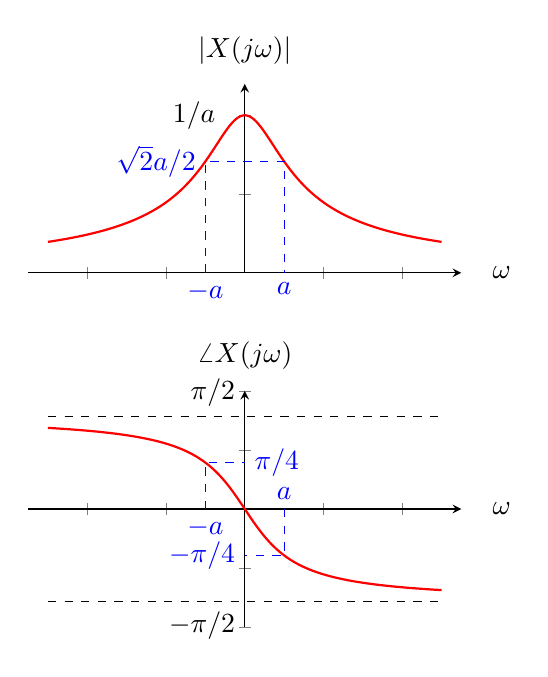
\begin{tikzpicture}[scale=1]
\begin{scope}	
    \begin{axis}[
		y=2cm,
		x=0.5cm,
		 clip=false,
		 xmin=-5.5,xmax=5.5,
		 xlabel= $\omega$,
		 ylabel={$|X(j\omega)|$},
		 ymin=0,ymax=1.2,
		 axis lines=middle,
         	%xtick={-5, -4, ..., 5},
		 %ytick={-1, 1},
		 yticklabels=\empty,
		 xticklabels=\empty,
		 every axis x label/.style={at={(ticklabel* cs:1.05)}, anchor=west,},
		every axis y label/.style={at={(ticklabel* cs:1.05)}, anchor=south,},
     ]
		%\addplot+[red, smooth, mark=none] table [x={n}, y={xn}] {periodic_square_fs_samples_of_envilope_gen.dat};
		\addplot [red, thick, domain=-5:5, samples=200] plot{1/sqrt(x*x + 1))};
		\node at (axis cs:-0.5, 1) [anchor=east] { $1/a$ };
		\draw[dashed, blue] (axis cs:-1, 0) node[anchor=north] { $-a$} -- (axis cs:-1, 0.707) node[anchor=east] { $\sqrt{2} a/2$} --  (axis cs:1, 0.707)  --  (axis cs:1, 0) node[anchor=north] { $a$} ;
    \end{axis}
\end{scope}

\begin{scope}[yshift=-4.5cm]	
    \begin{axis}[
		y=0.75cm,
		x=0.5cm,
		 clip=false,
		 xmin=-5.5,xmax=5.5,
		 xlabel= $\omega$,
		 ylabel={$\angle X(j\omega)$},
		 ymin=-2,ymax=2,
		 axis lines=middle,
         	%xtick={-5, -4, ..., 5},
		 %ytick={-1, 1},
		 yticklabels=\empty,
		 xticklabels=\empty,
		 every axis x label/.style={at={(ticklabel* cs:1.05)}, anchor=west,},
		every axis y label/.style={at={(ticklabel* cs:1.05)}, anchor=south,},
     ]
		%\addplot+[red, smooth, mark=none] table [x={n}, y={xn}] {periodic_square_fs_samples_of_envilope_gen.dat};
		\addplot [red, thick, domain=-5:5, samples=200] plot{-rad(atan(x))};
		\draw[dashed, blue] (axis cs:1, 0) node[anchor=south] { $a$} -- (axis cs:1, -pi/4)  -- (axis cs:0, -pi/4) node[anchor=east] { $-\pi/4$} ;
		\draw[dashed, blue] (axis cs:-1, 0) node[anchor=north] { $-a$} -- (axis cs:-1, pi/4)  -- (axis cs:0, pi/4) node[anchor=west] { $\pi/4$} ;
		\draw[dashed, black] (axis cs:-5, pi/2) --   (axis cs:5, pi/2) node[midway, anchor=south east] {$\pi/2$} ;
		\draw[dashed, black] (axis cs:-5, -pi/2) --   (axis cs:5, -pi/2) node[midway, anchor=north east] {$-\pi/2$} ;
   \end{axis}
\end{scope}
\end{tikzpicture} 
          \caption{Fourier transform of the signal $e^{-at}u(t), \quad a> 0$.}\label{fi:eatut}
        \end{figure}    
    }
\end{frame}

\begin{frame}
    \begin{example}
        Find the Fourier transform of the signal
        \begin{equation*}
            x(t) = e^{-a|t|}, \quad a> 0.
        \end{equation*}
    \end{example}
    \pause
    \mode<beamer>
    {
        \begin{equation*}
            \begin{aligned}
                X(j\omega) &= \int_{-\infty}^{\infty}x(t)e^{-j\omega t} dt.\\ \pause
                &= \int_{-\infty}^{\infty} e^{-a|t|} e^{-j\omega t} dt.\\ \pause
                X(j\omega) &= \int_{-\infty}^{0} e^{at}e^{-j\omega t}dt + \int_{0}^{\infty} e^{-at}e^{-j\omega t}dt\\ \pause
                X(j\omega) &= \frac{1}{a-j\omega} + \frac{1}{a+j\omega},\\
                &= \frac{2a}{a^2+\omega^2}.
            \end{aligned}
        \end{equation*}
    }
\end{frame}

\begin{frame}[plain]
    \mode<beamer>
    {
        \begin{figure}
          \centering
          \begin{tikzpicture}[scale=1]
\begin{scope}	
    \begin{axis}[
		y=1cm,
		x=1cm,
		 clip=false,
		 xmin=-5.5,xmax=5.5,
		 xlabel= $t$,
		 ylabel={$x(t)$},
		 ymin=0,ymax=1.2,
		 axis lines=middle,
         	%xtick={-5, -4, ..., 5},
		 %ytick={-1, 1},
		 yticklabels=\empty,
		 xticklabels=\empty,
		 every axis x label/.style={at={(ticklabel* cs:1.05)}, anchor=west,},
		every axis y label/.style={at={(ticklabel* cs:1.05)}, anchor=south,},
     ]
		%\addplot+[red, smooth, mark=none] table [x={n}, y={xn}] {periodic_square_fs_samples_of_envilope_gen.dat};
		\addplot [red, thick, domain=-5:5, samples=200] plot{exp(-abs(x))};
		\node at (axis cs:-0.5, 1) [anchor=east] { $1$ };
    \end{axis}
\end{scope}
\begin{scope}[yshift=-3.5cm]	
    \begin{axis}[
		y=1cm,
		x=1cm,
		 clip=false,
		 xmin=-5.5,xmax=5.5,
		 xlabel= $\omega$,
		 ylabel={$|X(j\omega)|$},
		 ymin=0,ymax=2.5,
		 axis lines=middle,
         	%xtick={-5, -4, ..., 5},
		 %ytick={-1, 1},
		 yticklabels=\empty,
		 xticklabels=\empty,
		 every axis x label/.style={at={(ticklabel* cs:1.05)}, anchor=west,},
		every axis y label/.style={at={(ticklabel* cs:1.05)}, anchor=south,},
     ]
		%\addplot+[red, smooth, mark=none] table [x={n}, y={xn}] {periodic_square_fs_samples_of_envilope_gen.dat};
		\addplot [red, thick, domain=-5:5, samples=200] plot{2/(x*x + 1))};
		\node at (axis cs:-0.5, 2) [anchor=east] { $2/a$ };
		\draw[dashed, blue] (axis cs:-1, 0) node[anchor=north] { $-a$} -- (axis cs:-1, 1) node[anchor=east] { $1/a$} --  (axis cs:1, 1)  --  (axis cs:1, 0) node[anchor=north] { $a$} ;
    \end{axis}
\end{scope}
\end{tikzpicture} 
          \caption{Fourier transform of the signal $e^{-a|t|}, \quad a> 0$.}\label{fi:eat}
        \end{figure}    
    }
\end{frame}




\begin{frame}
    \begin{example}
        Determine the Fourier transform of the unit impulse
        \begin{equation*}
            x(t) = \delta(t).
        \end{equation*}
    \end{example}
    \pause
    \mode<beamer>
    {
        \begin{equation*}
            X(j\omega) = \int_{-\infty}^{\infty} \delta(t)e^{-j\omega t} dt = 1.
        \end{equation*}
        The unit impulse has a Fourier transform consisting of qual contributions at all frequencies.
    }
\end{frame}


\begin{frame}
    \begin{example}
        Determine the Fourier transform of the signal
        \begin{equation*}
            x(t) = \begin{cases}
                1,& |t| < T_1,\\
                0, & |t| > T_1.
            \end{cases}
        \end{equation*}
    \end{example}
    \pause
    \mode<beamer>
    {
        \begin{figure}
          \centering
          \begin{tikzpicture}[scale=0.5]
\begin{scope}[xshift=-6cm, yshift=2cm]

	\def\xmin{-4}
	\def\xmax{4}
	\def\ymin{0}
	\def\ymax{2}
	\def\period{2.0}
	\def\T1{1}
	\def\A{1}
	
	\edef\pulse{|- ++(2*\T1, \A) |- ++( \period - \T1, -\A)}

	
	\draw (\xmin-1, 0) --(\xmax+1, 0) node[anchor=west] {\small $t$};
	\draw (0, \ymin) --(0, \ymax) node[anchor=south] {\small $x_1(t)$};
	\draw[thick] (-3, 0) -- (-\T1,0) -- (-\T1, 1) -- (\T1,1) -- (\T1,0) -- (3,0);
		
		\node at (-\T1, 0) [anchor=north] {\small $-T_1$};
		\node at (\T1, 0) [anchor=north] {\small $T_1$};
		\node at (0, 1) [anchor=south east] {\small $1$};

\end{scope}		
\begin{scope}	
    \begin{axis}[
		y=4cm,
		x=1cm,
		 clip=false,
		 xmin=-5.5,xmax=5.5,
		 xlabel= $\omega$,
		 ylabel={$X_1(j\omega)$},
		 ymin=-0.5,ymax=1.2,
		 axis lines=middle,
         	%xtick={-5, -4, ..., 5},
		 %ytick={-1, 1},
		 yticklabels=\empty,
		 xticklabels=\empty,
		 every axis x label/.style={at={(ticklabel* cs:1.05)}, anchor=west,},
		every axis y label/.style={at={(ticklabel* cs:1.05)}, anchor=south,},
     ]
		%\addplot+[red, smooth, mark=none] table [x={n}, y={xn}] {periodic_square_fs_samples_of_envilope_gen.dat};
		\addplot [red, thick, domain=-5:5, samples=200] plot{sin(pi*deg(x))/(pi*x)};
		\node at (axis cs:0, 1) [anchor=east] { $2T_1$ };
		\draw[latex-] (axis cs:pi/3, 0) --(axis cs:0.6,-0.3) node  [anchor=north] { $\pi/T_1$ } ;
		\draw[latex-] (axis cs:-pi/3, 0) --(axis cs:-0.6,-0.3) node  [anchor=north] { $-\pi/T_1$ } ;		
    \end{axis}
\end{scope}		
\end{tikzpicture}

          \caption{Rectangular pulse and the Fourier transform.}\label{fi:square_pulse}
        \end{figure} 
    }
\end{frame}

\begin{frame}
    \mode<beamer>
    {
        \begin{equation*}
            \begin{aligned}
                X(j\omega) &= \int_{-\infty}^{\infty}x(t)e^{-j\omega t} dt.\\ \pause
                &= \int_{-T_1}^{T_1} e^{-j\omega t} dt.\\ \pause
                &= \left.\frac{e^{-j\omega t}}{-j\omega}\right|_{-T_1}^{T_1} \\ \pause
                &= 2\frac{\sin \omega T_1}{\omega}.\\
            \end{aligned}
        \end{equation*}
    }
\end{frame}


\begin{frame}
    \begin{example}
        Consider the signal $x(t)$ whose Fourier transform is
        \begin{equation*}
            X(j\omega) = \begin{cases}
                1,& |\omega| < W,\\
                0, & |\omega| > W.
            \end{cases}
        \end{equation*}
        Determine $x(t)$.
        \begin{figure}
          \centering
          \begin{tikzpicture}
	\draw (-2,0) -- (2,0) node [anchor=west] {\scriptsize $\omega$};
	\draw (0,0) -- (0,2) node [anchor=south] {\scriptsize $X(j\omega)$};
	\draw[thick] (-1,0) node [anchor=north] {\scriptsize $-W$} |- (1,1) -- (1,0) node [anchor=north] {\scriptsize $W$};

\end{tikzpicture}
          \caption{Fourier transform for $x(t)$.}\label{fi:xomega_square}
        \end{figure}
    \end{example}
    \pause
    \mode<beamer>
    {
       
    }
\end{frame}



\begin{frame}[plain]
    \mode<beamer>
    {
    
        Using the synthesis equation:
        \begin{equation*}
            \begin{aligned}
                x(t) &= \frac{1}{2\pi}\int_{-\infty}^{\infty}X(j\omega)e^{j\omega t} d\omega.\\ \pause
                &= \frac{1}{2\pi}\int_{-W}^{W}e^{j\omega t} d\omega.\\ \pause
                &= \frac{\sin W t}{\pi t}.\\
            \end{aligned}
        \end{equation*} 
        \pause    
        \begin{figure}
          \centering
          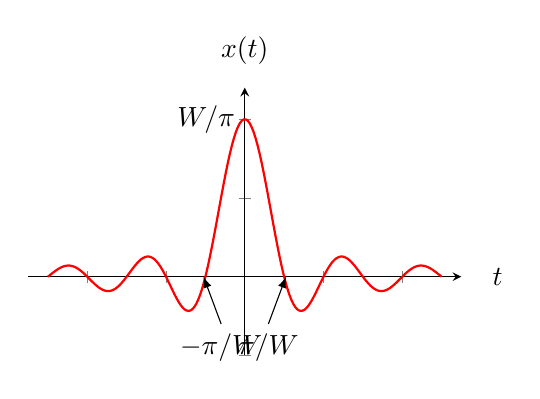
\begin{tikzpicture}
\begin{scope}	
    \begin{axis}[
		y=2cm,
		x=0.5cm,
		 clip=false,
		 xmin=-5.5,xmax=5.5,
		 xlabel= $t$,
		 ylabel={$x(t)$},
		 ymin=-0.5,ymax=1.2,
		 axis lines=middle,
         	%xtick={-5, -4, ..., 5},
		 %ytick={-1, 1},
		 yticklabels=\empty,
		 xticklabels=\empty,
		 every axis x label/.style={at={(ticklabel* cs:1.05)}, anchor=west,},
		every axis y label/.style={at={(ticklabel* cs:1.05)}, anchor=south,},
     ]
		%\addplot+[red, smooth, mark=none] table [x={n}, y={xn}] {periodic_square_fs_samples_of_envilope_gen.dat};
		\addplot [red, thick, domain=-5:5, samples=200] plot{sin(pi*deg(x))/(pi*x)};
		\node at (axis cs:0, 1) [anchor=east] { $W/\pi$ };
		\draw[latex-] (axis cs:pi/3, 0) --(axis cs:0.6,-0.3) node  [anchor=north] { $\pi/W$ } ;
		\draw[latex-] (axis cs:-pi/3, 0) --(axis cs:-0.6,-0.3) node  [anchor=north] { $-\pi/W$ } ;		
    \end{axis}
\end{scope}	
\end{tikzpicture} 
          \caption{Time function.}\label{fi:rectift}
        \end{figure}
    }
\end{frame}



\begin{frame}{The $\mathrm{sinc}$ Function}
    \begin{equation}\label{eq:sinc_function}
        \mathrm{sinc}(\theta) = \frac{\sin \pi \theta}{\pi \theta}.
    \end{equation}
    \begin{figure}
      \centering
      \begin{tikzpicture}
\begin{scope}	
    \begin{axis}[
		y=2cm,
		x=1cm,
		 clip=false,
		 xmin=-5.5,xmax=5.5,
		 xlabel= $\theta$,
		 ylabel={$\mathrm{sinc}(\theta)$},
		 ymin=-0.5,ymax=1.2,
		 axis lines=middle,
         	%xtick={-5, -4, ..., 5},
		 %ytick={-1, 1},
		 yticklabels=\empty,
		 every axis x label/.style={at={(ticklabel* cs:1.05)}, anchor=west,},
		every axis y label/.style={at={(ticklabel* cs:1.05)}, anchor=south,},
     ]
		%\addplot+[red, smooth, mark=none] table [x={n}, y={xn}] {periodic_square_fs_samples_of_envilope_gen.dat};
		\addplot [red, thick, domain=-5:5, samples=200] plot{sin(pi*deg(x))/(pi*x)};
		\node at (axis cs:0, 1) [anchor=east] { $1$ };
    \end{axis}
\end{scope}
\end{tikzpicture} 
      \caption{Fourier transform for $x(t)$.}\label{fi:sinc_function}
    \end{figure}
\end{frame}


\begin{frame}
    Express
    \begin{equation*}
        \frac{2 \sin \omega T_1}{\omega}
    \end{equation*}
    and
    \begin{equation*}
        \frac{\sin W t}{\pi t}
    \end{equation*}
    as $\mathrm{sinc}$ functions.
    \pause
    \mode<beamer>
    {
        \begin{equation*}
            \begin{aligned}
                \frac{2 \sin \omega T_1}{\omega} &= 2T_1 \mathrm{sinc}\left(\frac{\omega T_1}{\pi}\right)\\ \pause
                \frac{\sin W t}{\pi t} &= \frac{W}{\pi} \mathrm{sinc}\left(\frac{W t}{\pi}\right)\\ \pause
            \end{aligned}
        \end{equation*}
    }
\end{frame}

%\subsection{The Fourier Transform for Periodic Signals}

\begin{frame}{The Fourier Transform for Periodic Signals: Introduction}
    In the previous section, we studied the Fourier transform representation, paying attention to aperiodic signals. We can also develop \ftrs~for periodic signals. This allows us to consider periodic and aperiodic signals in a unified context. We can construct the \ft of a periodic signal directly from its \fsr .

    Consider a signal $x(t)$  with \ft~ $X(j\omega)$ that is a single impulse of area $2\pi$ at $\omega=\omega_0$, i.e.,
    \begin{equation}
        X(j\omega) = 2\pi \delta(\omega-\omega_0)
    \end{equation}
\end{frame}

\begin{frame}
    Let's determine the signal $x(t)$:
    \pause
    \mode<beamer>
    {
        \begin{equation*}
            \begin{split}
                x(t) &= \frac{1}{2\pi}\int_{-\infty}^{\infty} 2\pi \delta(\omega-\omega_0)e^{j\omega t} d\omega,\\
                &= e^{j\omega_0 t}.\\
            \end{split}
        \end{equation*}
        \pause
        More generally, if $X(j\omega)$ is of the form of a linear combination of impulses equally spaced in frequency, i.e.,
        \begin{equation}
             X(j\omega) = \sum_{k=-\infty}^{\infty}2\pi a_k \delta(\omega-k\omega_0)
        \end{equation}
        \pause
        then
        \begin{equation}
            x(t) = \sum_{k=-\infty}^{\infty}e^{jk\omega_0 t}.
        \end{equation}
        which is exactly the \fsr~ of a periodic signal. \\
        Thus, the \ft of a periodic signal with \fs~coefficients $\{a_k\}$ can be interpreted as a train of impulses occurring at the harmonically related frequencies and for which the area of the impulse at the $k$th harmonic frequency $k\omega_0$ is $2\pi$ times the $k$th \fs~coefficient $a_k$.
    }

\end{frame}


\begin{frame}[plain]
    \begin{example}
        Find the \ft of the square wave signal whose \fs~coefficients are
        \begin{equation*}
            a_k = \frac{\sin k \omega_0 T_1}{\pi k}.
        \end{equation*}
    \end{example}
\end{frame}


\begin{frame}[plain]
    \begin{equation*}
        X(j\omega) = \sum_{k=-\infty}^{\infty}\frac{2\sin k\omega_0 T_1}{k}\delta(\omega-k\omega_0).
    \end{equation*}
    \pause
    \begin{figure}
      \centering
      %% \begin{tikzpicture}[scale=0.5]
% \begin{scope}	
%     \begin{axis}[
% 		y=4cm,
% 		x=1cm,
% 		 clip=false,
% 		 xmin=-10,xmax=10,
% 		 xlabel= $\omega$,
% 		 ylabel={$X(j\omega)$},
% 		 ymin=-0.5,ymax=1.2,
% 		 axis lines=middle,
%          	%xtick={-5, -4, ..., 5},
% 		 %ytick={-1, 1},
% 		 yticklabels=\empty,
% 		 xticklabels=\empty,
% 		 every axis x label/.style={at={(ticklabel* cs:1.05)}, anchor=west,},
% 		every axis y label/.style={at={(ticklabel* cs:1.05)}, anchor=south,},
%      ]
% 		%\addplot+[red, smooth, mark=none] table [x={n}, y={xn}] {periodic_square_fs_samples_of_envilope_gen.dat};
% 		\addplot [red, dashed, domain=-10:10, samples=200] plot{2*sin(deg(x)*2*pi/8*2)/(pi*x)};
% 		\addplot [thick, blue, ->, ycomb, domain=-10:10] plot{2*sin(deg(x)*2*pi/8*2)/(pi*x)};
% 		\node at (axis cs:0, 1) [anchor=east] { $\pi$ };
% 		\draw[latex-] (axis cs:pi/3, 0) --(axis cs:0.6,-0.3) node  [anchor=north] { $\pi/W$ } ;
% 		\draw[latex-] (axis cs:-pi/3, 0) --(axis cs:-0.6,-0.3) node  [anchor=north] { $-\pi/W$ } ;		
%     \end{axis}
% \end{scope}	
% \end{tikzpicture} 

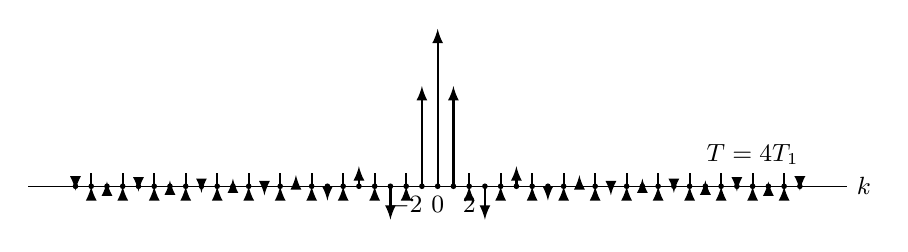
\begin{tikzpicture}[scale=0.4]
	\def\w{{-23,-22,-21,-20,-19,-18,-17,-16,-15,-14,-13,-12,-11,-10,-9,-8,-7,-6,-5,-4,-3,-2,-1,0,1,2,3,4,5,6,7,8,9,10,11,12,13,14,15,16,17,18,19,20,21,22,23}}
	\def\akmag{{-0.013840,0.000000,0.015158,-0.000000,-0.016753,0.000000,0.018724,-0.000000,-0.021221,0.000000,0.024485,-0.000000,-0.028937,0.000000,0.035368,-0.000000,-0.045473,0.000000,0.063662,-0.000000,-0.106103,0.000000,0.318310,0.500000,0.318310,0.000000,-0.106103,-0.000000,0.063662,0.000000,-0.045473,-0.000000,0.035368,0.000000,-0.028937,-0.000000,0.024485,0.000000,-0.021221,-0.000000,0.018724,0.000000,-0.016753,-0.000000,0.015158,0.000000,-0.013840}}


	\begin{scope}	
		\draw (-13, 0) -- (13,0) node[anchor=west] {\small $k$};
		\foreach \k in {-2, 0, 2}
		{
			\node at (\k/2, 0) [anchor=north] {\small $\k$};
		}
		%\node at (0,5) [anchor=south] {\small $Ta_k$};
		
		\foreach \k in {0,1, ..., 46}
		{
			\pgfmathparse{\w[\k]/2}
			\edef\wk{\pgfmathresult}
			\pgfmathparse{\akmag[\k]}
			\edef\akmagk{\pgfmathresult}	
			\draw[thick, -latex] (\wk, 0) -- ++(0,10*\akmagk);% node [anchor=south] {\small $\akmagk$};
			\ifthenelse{\lengthtest{0 pt = \akmagk pt}}{\draw[fill=black]  (\wk,0) circle (2pt);}{}
		}
			\node at (10, 1) {\small $T= 4T_1$};		
	\end{scope}
	\end{tikzpicture}
      \caption{Fourier transform of a symmetric periodic square wave.}\label{fi:ft_square_wave}
    \end{figure}
\end{frame}



\begin{frame}[plain]
    \begin{example}
        Find the \ft of
            \begin{equation*}
                x(t) = \sin \omega_0 t.
            \end{equation*}
            and
            \begin{equation*}
                x(t) = \cos \omega_0 t.
            \end{equation*}
    \end{example}
\end{frame}

\begin{frame}[plain]
    \begin{example}
        Find the \ft of the impulse train
        \begin{equation*}
            x(t) = \sum_{k=-\infty}^{\infty} \delta(t-kT).
        \end{equation*}
    \end{example}
\end{frame}



